%% Extraído de docs/TCC_documento/Textuais/Conclusao/01_Discussao.tex (linhas 104-128)
    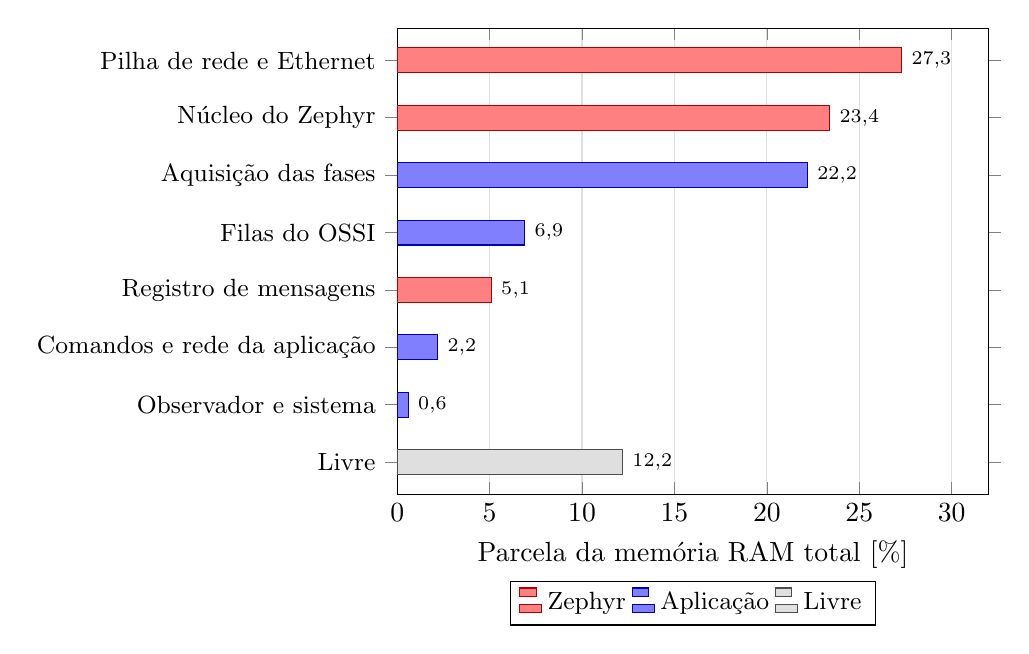
\begin{tikzpicture}
        \begin{axis}[
            xbar, bar width=9pt, bar shift=0pt, width=0.75\textwidth, height=7.5cm,
            legend style={at={(0.5,0)}, anchor=north, yshift=-1.1cm, legend columns=3, font=\small},
            xmin=0, xmax=32,
            xlabel={Parcela da memória RAM total [\%]},
            symbolic y coords={Livre, Observador e sistema, Comandos e rede da aplicação, Registro de mensagens, Filas do OSSI, Aquisição das fases, Núcleo do Zephyr, Pilha de rede e Ethernet},
            ytick={Livre, Observador e sistema, Comandos e rede da aplicação, Registro de mensagens, Filas do OSSI, Aquisição das fases, Núcleo do Zephyr, Pilha de rede e Ethernet},
            enlarge y limits=0.08,
            y tick label style={font=\small},
            nodes near coords={\pgfmathprintnumber[fixed, precision=1, use comma]{\pgfplotspointmeta}},
            nodes near coords style={font=\scriptsize},
            xmajorgrids, grid style={gray!25},
        ]
            \addplot[fill=red!50, draw=red!70!black] coordinates
                {(27.3,Pilha de rede e Ethernet) (23.4,Núcleo do Zephyr)
                 (5.1,Registro de mensagens)};
            \addplot[fill=blue!50, draw=blue!70!black] coordinates
                {(22.2,Aquisição das fases) (6.9,Filas do OSSI)
                 (2.2,Comandos e rede da aplicação) (0.6,Observador e sistema)};
            \addplot[fill=gray!25, draw=gray!60!black] coordinates
                {(12.2,Livre)};
            \legend{Zephyr, Aplicação, Livre}
        \end{axis}
    \end{tikzpicture}
